% Lecture Template for ME3001 - Mechanical Engineering Analysis - Tennessee Technological University
% Spring 2024 - condensing and streamlining lectures by combining topics into a single PDF under the module name
% this will simplify file and link management as well as make lectures easier to use in class
% - added image/ to clean directory and reduce redundancy, specific to module for now  

% Module Name: - Systems of Linear Equations
% Topic 1 - Linear Systems Review
% Topic 2 - Matrix Multiplication
% Topic 3 - Existence of Solutions
% Topic 4 - Gaussian Elimination

\documentclass[fleqn]{beamer} % for presentation (has nav buttons at bottom)

\usepackage{../analysis_lectures} % sty in the parent directory

\author{ME3001 - Mechanical Engineering Analysis}

\newcommand{\MNUM}{3\hspace{2mm}} % module number 
\newcommand{\moduletitle}{Systems of Linear Equations}

\newcommand{\sectionItitle}{Linear Systems Review}
\newcommand{\sectionIItitle}{Matrix Multiplication}
\newcommand{\sectionIIItitle}{Existence of Solutions}
\newcommand{\sectionIVtitle}{Gaussian Elimination}

\newcommand{\sectionIsubsectionItitle}{What is a Linear Equation ?}
\newcommand{\sectionIsubsectionIItitle}{General Form of  A Linear System}
\newcommand{\sectionIsubsectionIIItitle}{The Geometrical Explanation}
\newcommand{\sectionIsubsectionIVtitle}{Examples in MATLAB}

\newcommand{\sectionIIsubsectionItitle}{Motivation}
\newcommand{\sectionIIsubsectionIItitle}{Multiplication of Conformible Matrices}
\newcommand{\sectionIIsubsectionIIItitle}{Generalized Description of Multiplication}
\newcommand{\sectionIIsubsectionIVtitle}{Exercise in MATLAB}

\newcommand{\sectionIIIsubsectionItitle}{Techniques for Solving Linear Systems}
\newcommand{\sectionIIIsubsectionIItitle}{Homogeneous and Inhomogeneous Systems}
\newcommand{\sectionIIIsubsectionIIItitle}{Solution Existence Cases in 2D}
\newcommand{\sectionIIIsubsectionIVtitle}{Numerical Error and System Condition}

\newcommand{\sectionIVsubsectionItitle}{Various Row-Reduction Methods}
\newcommand{\sectionIVsubsectionIItitle}{Gaussian Elimination Technique}
\newcommand{\sectionIVsubsectionIIItitle}{A Generalized Algorithm}
\newcommand{\sectionIVsubsectionIVtitle}{}

% custom box
\newsavebox{\mybox}

\title{Lecture Module - \moduletitle}

\date{Mechanical Engineering\vspc Tennessee Technological University}

\begin{document}

	\lstset{language=MATLAB,basicstyle=\ttfamily\small,showstringspaces=false}

	\frame{\titlepage \center\begin{framed}\Large \textbf{Module \MNUM - \moduletitle}\end{framed} \vspace{5mm}}

	% Module Outline
	\begin{frame} 
		\large \textbf{Module \MNUM - \moduletitle} \vspace{3mm}\\

		\begin{itemize}
			\item Topic 1 - \hyperlink{sectionI}{\sectionItitle} \vspc % section I
			\item Topic 2 - \hyperlink{sectionII}{\sectionIItitle} \vspc % section II
			\item Topic 3 - \hyperlink{sectionIII}{\sectionIIItitle} \vspc % section III
		\end{itemize}

	\end{frame}

	% section I
	\section{\sectionItitle}\label{sectionI}

		% section I Outline
		\begin{frame} 
			\large \textbf{Topic 1 - \sectionItitle} \vspace{3mm}\\

			\begin{itemize}
				\item \hyperlink{sectionIsubsectionI}{\sectionIsubsectionItitle} \vspc %  section I subsection I
				\item \hyperlink{sectionIsubsectionII}{\sectionIsubsectionIItitle} \vspc % section I subsection II
				\item \hyperlink{sectionIsubsectionIII}{\sectionIsubsectionIIItitle} \vspc % section I subsection III
				\item \hyperlink{sectionIsubsectionIV}{\sectionIsubsectionIVtitle} \vspc % section I subsection IV
			\end{itemize}
		\end{frame}
		
		% section I subsection I 
		\subsection{\sectionIsubsectionItitle}\label{sectionIsubsectionI}

			\begin{frame}
				\frametitle{\sectionIsubsectionItitle}
				\bigskip

				\textbf{What is a Linear Equation}

				\begin{itemize}
					\item ``A linear equation is an algebraic equation in which each term is either a constant or the product of a constant and a single variable'' - Wikipedia \vspace{3mm}\\
					\item slope intercept form	\vspace{3mm}\\
					\item does not contain \vspace{3mm}\\
				\end{itemize}	

				\textbf{ What is a System of Linear Equations?}
				\begin{itemize}
					\item multiple linear equations with... \vspace{3mm}\\
					\item also known as... \vspace{3mm}\\		
				\end{itemize}

				\btVFill
			\end{frame}

		% section I subsection II
		\subsection{\sectionIsubsectionIItitle}\label{sectionIsubsectionII}

			\begin{frame}
				\frametitle{\sectionIsubsectionIItitle} \small
				\bigskip

				\begin{fleqn}
		
					The general system of linear equations  is shown with variables $x_{1,2,..,n}$ , coefficients $a_{11,12,..,nm}$, and knowns $b_{1,2,...,m}$ \vspace{1mm}\\		  
					
					\[a_{11} x_1 + a_{12} x_{2} + ... + a_{1n} x_n = b_1 \] 
					\[a_{21} x_1 + a_{22} x_{2} + ... + a_{2n} x_n = b_2 \] 
					\[\hspace{20mm}.\]		
					\[a_{m1} x_1 + a_{m2} x_{2} + ... + a_{mn} x_n = b_m \]			

				\end{fleqn}  

				The equations are cast into matrix form of the system. 	\\
				\begin{fleqn}

					\[ \left( \begin{array}{cccc}
					a_{11} & a_{12} & ...& a_{1n} \\
					a_{21} & a_{22} & ...& a_{2n} \\
					&.&&\\
					&.&&\\
					a_{m1} & a_{m2} & ...& a_{mn}\end{array} \right) \times \left[ \begin{array}{c}
					x_1 \\
					x_2 \\
					.\\
					.\\
					x_n \end{array} \right] = \left[ \begin{array}{c}
					b_1 \\
					b_2 \\
					.\\
					.\\
					b_m \end{array} \right]\] 

				\end{fleqn}

				\btVFill
			\end{frame}

				%\btVFill
			\begin{frame}
				\frametitle{\sectionIsubsectionIItitle} \small
				\bigskip

				To verify the matrix form $[A]\{x\}=\{b\}$ is correct, use matric multiplication and the result will match the individual equations.	

				\begin{fleqn}

					\[ \left( \begin{array}{cccc}
					a_{11} & a_{12} & ...& a_{1n} \\
					a_{21} & a_{22} & ...& a_{2n} \\
					&.&&\\
					&.&&\\
					a_{m1} & a_{m2} & ...& a_{mn}\end{array} \right) \times \left[ \begin{array}{c}
					x_1 \\
					x_2 \\
					.\\
					.\\
					x_n \end{array} \right] = \left[ \begin{array}{c}
					b_1 \\
					b_2 \\
					.\\
					.\\
					b_m \end{array} \right]\] 

				\end{fleqn}


				\btVFill
			\end{frame}

		% section I subsection III
		\subsection{\sectionIsubsectionIIItitle}\label{sectionIsubsectionIII}
			\begin{frame} 
				\frametitle{\sectionIsubsectionIIItitle}
				\bigskip

				 Consider the intersection of two Lines on the XY plane (2D).  \hspace{5mm} 

					\begin{itemize}
	
						\item Write an equation for each line.  $ax+by=c$ \vspace{3mm} \\
	
						\item Organize the equations. \vspace{3mm} \\
					
					\end{itemize}

				\btVFill
			\end{frame}	

			\begin{frame} 
				\frametitle{\sectionIsubsectionIIItitle}
				\bigskip

			 	Consider the intersection of two Lines on the XY plane (2D).  \hspace{5mm} 
  
				\begin{itemize}
		
					\item Cast the system into matrix form. \vspace{10mm}
			
					\item Solve the system. What exactly does this mean?\\
				
					\begin{itemize}
							\item \hspace{10mm} \\
							\item \hspace{10mm} \\
							\item \hspace{10mm} \\
					\end{itemize}
			
				\end{itemize}
	
				\btVFill
			\end{frame}	

			\begin{frame} 
				\frametitle{\sectionIsubsectionIIItitle}
				\bigskip

		 		Repeat the exercise, and now consider the intersection of three planes in space (3D). What does the solution represent?  \hspace{3mm} \\ 
  
				\begin{itemize}
		
					\item Write an equation for each plane.  $ax+by+cz=d$ \vspace{3mm} \\
		
					\item Organize the equations. \vspace{3mm} \\
				\end{itemize}
				
				\btVFill
			\end{frame}	

			\begin{frame} 
				\frametitle{\sectionIsubsectionIIItitle}
				\bigskip
	
				\begin{itemize}
		
					\item Cast the system into matrix form. \vspace{10mm}
			
					\item Solve the system. What exactly does this mean?\\
					\begin{itemize}
						\item \hspace{10mm} \\
						\item \hspace{10mm} \\
						\item \hspace{10mm} \\
					\end{itemize}
		
				\end{itemize}
			
				\btVFill
			\end{frame}	



		% section I subsection IV
		\subsection{\sectionIsubsectionIVtitle}\label{sectionIsubsectionIV}	

			\begin{frame}
				\frametitle{\sectionIsubsectionIVtitle}
				\bigskip


				\btVFill
			\end{frame}
	
	% Section II
	\section{\sectionIItitle}\label{sectionII}

		% section II Outline
		\begin{frame}
			\large \textbf{Topic 2 - \sectionIItitle} \vspace{3mm}\\

			\begin{itemize}
				\item \hyperlink{sectionIIsubsectionI}{\sectionIIsubsectionItitle} \vspc %  section II subsection I
				\item \hyperlink{sectionIIsubsectionII}{\sectionIIsubsectionIItitle} \vspc % section II subsection II
				\item \hyperlink{sectionIIsubsectionIII}{\sectionIIsubsectionIIItitle} \vspc % section II subsection III
				\item \hyperlink{sectionIIsubsectionIV}{\sectionIIsubsectionIVtitle} \vspc % section II 
			\end{itemize}

		\end{frame}

		% section II subsection I
		\subsection{\sectionIIsubsectionItitle}\label{sectionIIsubsectionI}

			\begin{frame}[label=sectionIIsubsectionI]
				\frametitle{\sectionIIsubsectionItitle}
				\bigskip

				\begin{itemize}

					\item Why do we need to multiply matrices? \vspace{20mm}\\
	
					\item Why do we need to use a computer?
	
	  			\end{itemize}
  
				\btVFill
			\end{frame}

			\begin{frame}[label=sectionIIsubsectionI]
				\frametitle{\sectionIIsubsectionItitle}
				\bigskip

				Applications of Matrix Multiplication:
				\begin{itemize}
					\item

					\item

					\item	
				\end{itemize}

				\btVFill
			\end{frame}	

			\begin{frame}[label=sectionIIsubsectionI]
				\frametitle{\sectionIIsubsectionItitle}
				\bigskip

				
				\btVFill
			\end{frame}

		% section II subsection II
		\subsection{\sectionIIsubsectionIItitle}\label{sectionIIsubsectionII}

			\begin{frame}
				\frametitle{\sectionIIsubsectionIItitle} \small
				\bigskip

				Consider 2 conformable matrices $F$ and $G$ with elements $f_{ij}$ and $g_{ij}$. Matrix Multiplication gives the product matrix $E$ with elements $e_{ij}$.\vspace{0mm} 
		 
		 		\[E = F \times G \hspace{20mm} e_{ij}=\Sigma_{k=1}^n f_{ik}\times g_{kj}\] 
			 
				%	Here is an example with a two small matrices. \\
				%\begin{fleqn}		 
				\[
				\left[ \begin{array}{cc}
				e_{11} & e_{12}  \\
				e_{21} & e_{22}  \end{array} \right]=	 	
		 		\left[ \begin{array}{ccc}
				f_{11} & f_{12} & f_{13} \\
				f_{21} & f_{22} & f_{23} \end{array} \right] \times \left[ \begin{array}{cc}
				g_{11}&g_{12} \\
				g_{21}&g_{22} \\
				g_{31}&g_{32} \end{array} \right] 
				\]
				%\end{fleqn}	

				\btVFill 
			\end{frame}	

			\begin{frame}
				\frametitle{\sectionIIsubsectionIItitle} \small
				\bigskip

				\btVFill
			\end{frame}		


		% section II subsection III
		\subsection{\sectionIIsubsectionIIItitle}\label{sectionIIsubsectionIII}

			\begin{frame}
				\frametitle{\sectionIIsubsectionIIItitle} \small
				\bigskip


				\begin{fleqn}		 
				\[ e_{ij}=\Sigma_{k=1}^n f_{ik}\times g_{kj} \]
	 
					\[
					\left[ \begin{array}{cc}
					e_{11} & e_{12}  \\
					& \\ 
					e_{21} & e_{22}  \end{array}	\right]=\left[ \begin{array}{c|c}
					f_{11}g_{11}+f_{12}g_{21}+f_{13}g_{31} & f_{11}g_{12}+f_{12}g_{22}+f_{13}g_{32}  \\
					& \\ 
					f_{21}g_{11}+f_{22}g_{21}+f_{23}g_{31} & f_{21}g_{12}+f_{22}g_{22}+f_{23}g_{32}  \end{array}	\right]
					\]
		 
				\end{fleqn}	

				\begin{itemize}
		
					\item What does that equation above mean? \\
					\item How can we write a {\it General Solution Technique} using the equation?
			
				\end{itemize}

				
				\btVFill 
			\end{frame}

			\begin{frame}
				\frametitle{\sectionIIsubsectionIIItitle}\small
				\bigskip



				\btVFill 
			\end{frame}


		% section II subsection IV 
		\subsection{\sectionIIsubsectionIVtitle}\label{sectionIIsubsectionIV}

			\begin{frame}
				\frametitle{\sectionIIsubsectionIVtitle}
				\bigskip

				\textbf{A Programming Exercise - Matrix Multiplication}\\	


				\btVFill 
			\end{frame}

			\begin{frame}
				\frametitle{\sectionIIsubsectionIVtitle}
				\bigskip


				\btVFill 
			\end{frame}
		
	% Section III
	\section{\sectionIIItitle}\label{sectionIII}

		% section III Outline
		\begin{frame}
			\large \textbf{Topic 3 - \sectionIIItitle} \vspace{3mm}\\

			\begin{itemize}
				\item \hyperlink{sectionIIIsubsectionI}{\sectionIIIsubsectionItitle} \vspc %  section III subsection I
				\item \hyperlink{sectionIIIsubsectionII}{\sectionIIIsubsectionIItitle} \vspc % section III subsection II
				\item \hyperlink{sectionIIIsubsectionIII}{\sectionIIIsubsectionIIItitle} \vspc % section III subsection III
				\item \hyperlink{sectionIIIsubsectionIV}{\sectionIIIsubsectionIVtitle} \vspc % section III subsection IV
			\end{itemize}

		\end{frame}

		% section III subsection I
		\subsection{\sectionIIIsubsectionItitle}\label{sectionIIIsubsectionI}

			\begin{frame}
				\frametitle{\sectionIIIsubsectionItitle}
				\bigskip

				\textbf{There are many different techniques for solving linear systems. This is not an exhaustive list.} \\	
				\begin{itemize}
					\item Kramer's Method
					\item Gaussian Elimination 
					\item Gauss-Seidel Method
					\item Jacobi Method
				\end{itemize}
			  	
				\btVFill
			\end{frame}

			\begin{frame}
				\frametitle{\sectionIIIsubsectionItitle}
				\bigskip

			  
				\btVFill
			\end{frame}

		% section III subsection II
		\subsection{\sectionIIIsubsectionIItitle}\label{sectionIIIsubsectionII}	

			\begin{frame}
				\frametitle{\sectionIIIsubsectionIItitle}
				\bigskip

				\textbf{ Not all problems can be solved with this type of technique!} \vspace{3mm}\\	
				\begin{itemize}
					\item {\PR non-homogeneous} system is one in which ... \vspace{10mm}\\
					\item most of the time the system will be {\PR non-homogeneous} \vspace{10mm}\\
					\item a {\PR non-homogeneous} system has a {\BL proper solution} if and only if\vspace{2mm}\\
					\[rank(A)=rank([A | b])=n\]
				\end{itemize}
				
				\btVFill
			\end{frame}

			\begin{frame}
				\frametitle{\sectionIIIsubsectionIItitle}
				\bigskip
				

				\btVFill
			\end{frame}

		% section III subsection III
		\subsection{\sectionIIIsubsectionIIItitle}\label{sectionIIIsubsectionIII}

			\begin{frame}
				\frametitle{\sectionIIIsubsectionIIItitle}
				\bigskip

				{\bf Normal Case - 2 Equations - 2 Unknowns - 1 Solution} \\ \vspace{2mm}
				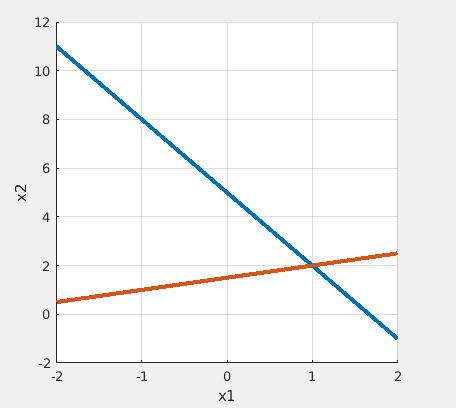
\includegraphics[scale=.3]{images/lecture5_fig1.png} \\
				\begin{fleqn}
					\[3x_1+x_2=5\]
					\[x_1-2x_2=-3\]
				\end{fleqn}

				\btVFill
			\end{frame}

			\begin{frame}
				\frametitle{\sectionIIIsubsectionIIItitle}
				\bigskip

				{\bf Abnormal Case - 2 Equations - 2 Unknowns - $\infty$ Solutions}  \\ \vspace{2mm}
				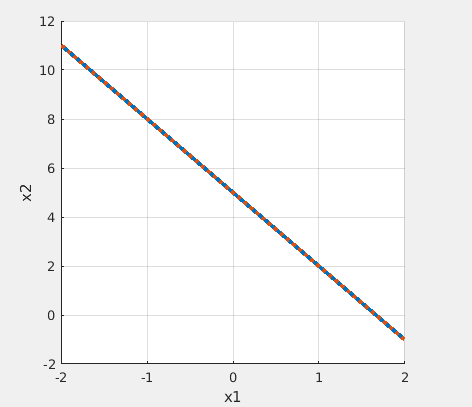
\includegraphics[scale=.3]{images/lecture5_fig2.png} \\
				\begin{fleqn}
					\[3x_1+x_2=5\]
					\[6x_1+2x_2=10\]
				\end{fleqn}

				\btVFill
			\end{frame}

			\begin{frame}
				\frametitle{\sectionIIIsubsectionIIItitle}
				\bigskip

				{\bf Abnormal Case - 2 Equations - 2 Unknowns - 0 Solutions} \\ \vspace{2mm}
				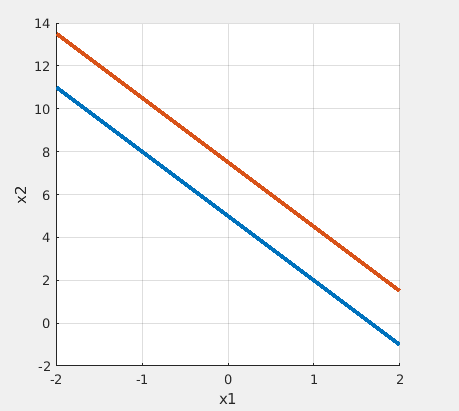
\includegraphics[scale=.3]{images/lecture5_fig3.png} \\
				\begin{fleqn}
					\[3x_1+x_2=5\]
					\[6x_1+2x_2=15\]
				\end{fleqn}

				\btVFill
			\end{frame}

			\begin{frame}
				\frametitle{\sectionIIIsubsectionIIItitle}
				\bigskip

				{\bf Abnormal Case - 3 Equations - 2 Unknowns - 0 Solutions} \\ \vspace{2mm}
				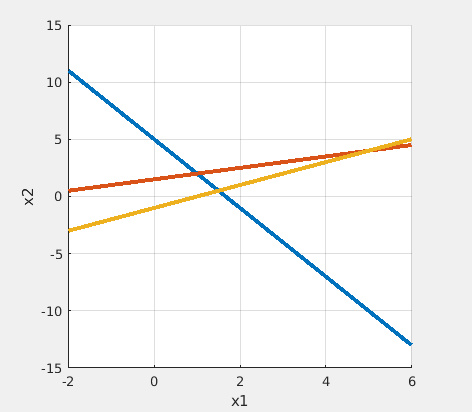
\includegraphics[scale=.3]{images/lecture5_fig4.png} \\
				\begin{fleqn}
				\[3x_1+x_2=5\]
				\[x_1-2x_2=-3\]
				\[x_1-x_2=1\]
				\end{fleqn}

				\btVFill
			\end{frame}

			\begin{frame}
				\frametitle{\sectionIIIsubsectionIIItitle}
				\bigskip

				{\bf Abnormal Case - 3 Equations - 2 Unknowns - 1 Solution} \\ \vspace{2mm}
				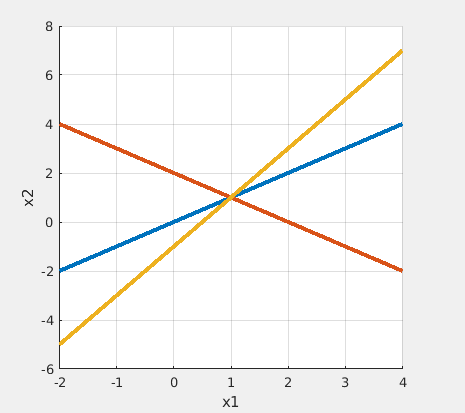
\includegraphics[scale=.3]{images/lecture5_fig5.png} \\
				\begin{fleqn}
				\[-x_1+x_2=0\]
				\[x_1+x_2=2\]
				\[-2x_1+x_2=-1\]
				\end{fleqn}

				\btVFill
			\end{frame}

			\begin{frame}
				\frametitle{\sectionIIIsubsectionIIItitle}
				\bigskip

				What happened to the summary table?

				\btVFill
			\end{frame}


		% section III subsection IV
		\subsection{\sectionIIIsubsectionIVtitle}\label{sectionIIIsubsectionIV}

			\begin{frame}
				\frametitle{\sectionIIIsubsectionIVtitle}
				\bigskip

				\textbf{We want our answer to have as little \scalebox{1.5}{error} as possible.} \vspace{3mm}\\

				\textbf{What causes error in the numerical methods?} \\
				``In software engineering and mathematics, numerical error is the combined effect of two kinds of error in a calculation. The first is caused by the finite precision of computations involving floating-point or integer values. The second usually called truncation error is the difference between the exact mathematical solution and the approximate solution obtained when simplifications are made to the mathematical equations to make them more amenable to calculation.''-wikipedia\\

				\btVFill
			\end{frame}	

			\begin{frame}
				\frametitle{\sectionIIIsubsectionIVtitle} \small
				\bigskip

				\textbf{Major Causes of Error} \\
				\begin{itemize}
					\item \textbf{floating point computations} \vspace{3mm}\\
					\item \textbf{truncation and solution simplification} \vspace{3mm}\\
					\item \textbf{system condition} \vspace{3mm}\\
					\item \textbf{lack of sleep...} \vspace{3mm}\\
				\end{itemize}
				
				\textbf{ The {\BL System Condition} can cause problems!} \\
				\begin{itemize}
				\item An {\PR ill-conditioned} system can cause error. \\
				\item A system is {\PR ill-conditioned} if small changes in the coefficients on the either side of the equation create large variations in the solution.\\
				\end{itemize}

				\btVFill
			\end{frame}	

			\begin{frame}
				\frametitle{\sectionIIIsubsectionIVtitle}
				\bigskip

				\begin{fleqn}
				  
				  	Consider this simple 2x2 example. The solution will have huge variations if $ k\approx 1 $. \\
				
					\[x_1 - x_2=5\] 
					\[kx_1 - x_2=4\]
				
				  	When $ k = 0.99 $, this gives a solution $(x_1,x_2)=(100, 95)$	
				
					\[x_1 - x_2=5\] 
					\[(0.99)x_1 - x_2=4\]
				
				 	When $ k = 1.01 $, this gives a solution $(x_1,x_2)=(-100, 105)$	
				
					\[x_1 - x_2=5\] 
					\[(1.01)x_1 - x_2=4\]
					
				\end{fleqn}

				\btVFill
			\end{frame}	
	


	% Section IV
	\section{\sectionIVtitle}\label{sectionIV}

		% section IV Outline
		\begin{frame}
			\large \textbf{Topic 3 - \sectionIVtitle} \vspace{3mm}\\

			\begin{itemize}
				\item \hyperlink{sectionIVsubsectionI}{\sectionIVsubsectionItitle} \vspc %  section IV subsection I
				\item \hyperlink{sectionIVsubsectionII}{\sectionIVsubsectionIItitle} \vspc % section IV subsection II
				\item \hyperlink{sectionIVsubsectionIII}{\sectionIVsubsectionIIItitle} \vspc % section IV subsection III
				\item \hyperlink{sectionIVsubsectionIV}{\sectionIVsubsectionIVtitle} \vspc % section IV subsection IV
			\end{itemize}

		\end{frame}

		% section IV subsection I
		\subsection{\sectionIVsubsectionItitle}\label{sectionIVsubsectionI}

			\begin{frame}
				\frametitle{\sectionIVsubsectionItitle}
				\bigskip

				The Gaussian Elimination method has many variations.  You may have used a different version in linear algebra, but that is fine. This method in generalized so that is can be automated easily with a computer program.   

				\btVFill
			\end{frame}

			\begin{frame}
				\frametitle{\sectionIVsubsectionItitle}
				\bigskip


				\btVFill
			\end{frame}

		% section IV subsection II
		\subsection{\sectionIVsubsectionIItitle}\label{sectionIVsubsectionII}

			\begin{frame}
				\frametitle{\sectionIVsubsectionIItitle}
				\bigskip

					The Gaussian Elimination consists of two main steps. Some variations of the method combine the two steps into a single procedure. \vspace{10mm}
  
			  	\begin{enumerate}

			    	\item Forward Elimination of Unknowns
			    
			    	\item Backwards Substitution   
			  
			  	\end{enumerate} 


				\btVFill
			\end{frame}

			\begin{frame}
				\frametitle{\sectionIVsubsectionIItitle}
				\bigskip

				\underline{{\bf Step 1:} Forward Elimination of Unknowns}
		
				\begin{itemize}
					\item  Eliminate $x_1$ from equations $2$ to $n$
						\begin{itemize}
							\item Eliminate $x_1$ from equation $2$
								\begin{itemize}
									\item define the eliminating factor $f_{21}$ as $a_{21}/a_{11}$
									\item redefine $a_{21}$ as $a_{21}-a_{11}*f_{21}$
									\item redefine $a_{22}$ as $a_{22}-a_{12}*f_{21}$ \\
									. . . 
									\item redifine $a_{2n}$ as $a_{2n}-a_{1n}*factor$ \\
								\end{itemize}
							\item Eliminate $x_1$ from equation $3$
								\begin{itemize}
									\item define the eliminating factor $f_{31}$ as $a_{31}/a_{11}$
									\item redefine $a_{31}$ as $a_{31}-a_{11}*f_{31}$
									\item redefine $a_{32}$ as $a_{32}-a_{12}*f_{31}$ \\
									 . . .
									\item redefine $a_{3n}$ as $a_{3n}-a_{1n}*f_{31}$ \\
								\end{itemize}	
						\end{itemize}
				\end{itemize}

				\btVFill
			\end{frame}	

			\begin{frame}
				\frametitle{\sectionIVsubsectionIItitle}
				\bigskip

				\begin{itemize}				
				\item   Eliminate $x_2$ from equations $3$ to $n$ \\
				\begin{itemize}
						\item Eliminate $x_2$ from equation $3$
					\begin{itemize}
						\item define the eliminating factor $f_{32}$ as $a_{32}/a_{22}$
						\item redefine $a_{32}$ as $a_{32}-a_{22}*f_{32}$
						\item redefine $a_{33}$ as $a_{33}-a_{23}*f_{32}$\\
						. . .
						\item redefine $a_{3n}$ as $a_{3n}-a_{2n}*f_{32}$ \\
						
					\end{itemize}
				
				\end{itemize}	
				. . . 
				%\renewcommand\labelitemiii{\textperiodcentered}
				\item   Eliminate $x_{n-1}$ from equation $n$ 

					\begin{itemize}
						\item define the eliminating factor $f_{n,n-1}$ as $a_{n,n-1}/a_{n-1,n-1}$
						\item redefine $a_{n,n-1}$ as $a_{n,n-1}-a_{n-1,n-1}*f_{n,n-1}$
						
					\end{itemize}
		
				\end{itemize}    

				\btVFill
			\end{frame}	


			\begin{frame}
				\frametitle{\sectionIVsubsectionIItitle}
				\bigskip

				 {\bf Step 2:} Backwards Subsitution
		%		\renewcommand\labelitemi{\textbullet}
		% 		\renewcommand\labelitemii{\textendash}
		% 		\renewcommand\labelitemiii{\textasteriskcentered}
		% 		\renewcommand\labelitemiv{\textperiodcentered}
				\begin{itemize}
					\item Solve Equations $n$ through $1$ \\
						\begin{itemize}
							\item Solve for $x_n$ as $\frac{b_n}{a_{n,n}}$\\
					
							\item Solve for $x_{n-1}$ as $\frac{b_{n-1}-(a_{n-1,n}x_n)}{a_{n-1,n-1}}$ \\
							
							\item Solve for $x_{n-2}$ as $\frac{b_{n-2}-(a_{n-2,n-1}x_{n-1})-(a_{n-2,n}x_{n})}{a_{n-2,n-2}}$\\
							. \\ .\\ . \\					 
							\item Solve for $x_{1}$ as $\frac{b_{1}-(a_{12}x_{2})- . . . -(a_{1,n-1}x_{n-1})-(a_{1,n}x_{n})}{a_{1,1}}$\\	
									
						\end{itemize}
				\end{itemize}

				\btVFill
			\end{frame}	

		% section IV subsection III
		\subsection{\sectionIVsubsectionIIItitle}\label{sectionIVsubsectionIII}

			\begin{frame}
				\frametitle{\sectionIVsubsectionIIItitle}
				\bigskip

				\begin{multicols}{2}
				\underline{{\bf Step 1:} Forward Elimination} \vspace{2mm}\\ 

		{\it for} \color{mypurple}k \color{black} {\it from} 1 {\it to} \color{mygreen}n\color{black}-1 \vspace{1mm}
	
		\hspace{3mm} {\it for} \color{blue}i \color{black} {\it from} \color{mypurple}k\color{black}+1 {\it to} \color{mygreen}n\color{black} \vspace{1mm}
		
		\hspace{6mm} fact$=a_{\color{blue}i\color{black},\color{mypurple}k}/a_{\color{mypurple}k\color{black},\color{mypurple}k\color{black}}$ \vspace{1mm}

		\hspace{9mm} {\it for} \color{red}j \color{black} {\it from} \color{mypurple} k \color{black}  {\it to} \color{mygreen}n\color{black} \vspace{1mm}

		\hspace{12mm} $a_{\color{blue}i\color{black},\color{red}j}=a_{\color{blue}i\color{black},\color{red}j}-fact\times a_{\color{mypurple}k\color{black},\color{red}j}$ \vspace{1mm}
		
\hspace{10mm}{\it end} \vspace{1mm}

\hspace*{9mm}$b_{\color{blue}i\color{black}}=b_{\color{blue}i\color{black}}-fact\times b_{\color{mypurple}k\color{black}}$ \vspace{1mm}

\hspace*{6mm}{\it end} \vspace{1mm}

{\it end}\vspace{15mm}
		%\hspace*{20mm} \scalebox{1.5}{\color{blue} end \color{black} }\\
		%\hspace{0mm} \scalebox{1.5}{\color{blue} end \color{black}}\\ \\
		%\hspace{0mm} \scalebox{1.5}{\color{blue} end \color{black}}\\
		
		\underline{{\bf Step 2:} Backwards Substitution} \vspace{2mm}
		
				$x_{\color{mygreen}n\color{black}}=b_{\color{mygreen}n\color{black}}/a_{\color{mygreen}n\color{black},\color{mygreen}n\color{black}}$ \vspace{2mm}
				
		{\it for} \color{blue}i \color{black} {\it from} \color{mygreen}n\color{black}-1 {\it to} 1 \vspace{4mm}
	
		\hspace*{10mm}$x_{\color{blue}i}=(b_{\color{blue}i}-\sum\limits^n_{\color{red}j\color{black}=\color{blue}i\color{black}+1}\left( a_{\color{blue}i\color{black},\color{red}j}x_{\color{red}j}\right)) /a_{\color{blue}i\color{black},\color{blue}i\color{black}}$	\vspace{2mm}
		
		{\it end} \vspace{2mm}
		
				\end{multicols}

				
				\btVFill
			\end{frame}	

\end{document}





